%\section[\hspace{-0.14in}El Modelo Estándar Cosmológico]{El Modelo Estándar Cosmológico}
\section*{El Modelo Estándar Cosmológico}

Nuestro Universo parece homogéneo e isotrópico a gran escala. Por esta razón, los modelos cosmológicos basados en la Relatividad General describen su geometría y evolución en términos de dos parámetros cosmológicos, es decir, la curvatura espacial $\kappa$ y el factor de escala $R(t)$, como se puede ver en la métrica de Robertson-Walker
\begin{equation}
ds^2 = dt^2 - R^2(t) \left[  \frac{dr^2}{1-\kappa r^2} + r^2 (d\theta^2 + \sin^2 \theta d\phi^2)  \right].
\label{RWmetric}
\end{equation}


Las ecuaciones cosmológicas del movimiento surgen de las ecuaciones de Einstein
\begin{equation}
R_{\mu \nu} - \frac{1}{2} g_{\mu \nu} R = 8 \pi G T_{\mu \nu} + \Lambda g_{\mu \nu} ,
\end{equation}
donde $R_{\mu \nu}$ es el tensor de Ricci definido por
\begin{equation}
R_{\mu \nu} = \partial_\lambda \Gamma^\lambda_{\mu \nu} - \partial_\mu \Gamma^\lambda_{\nu \lambda} + \Gamma^\lambda_{\mu \nu} \Gamma^\sigma_{\lambda \sigma} -  \Gamma^\lambda_{\mu \sigma} \Gamma^\sigma_{\lambda \nu},
\end{equation} 
los símbolos de Christoffel $\Gamma^\mu_{\nu \lambda}$ están definidos por
\begin{equation}
\Gamma^\mu_{\nu \lambda} = \frac{1}{2} g^{\mu \rho} (\partial_\nu g_{\rho \lambda}  + \partial_\lambda g_{\rho \nu} - \partial_\rho g_{\nu \lambda} ), 
\end{equation}
$g_{\mu \nu}$ es la métrica del espacio-tiempo, $R = g^{\mu \nu} R_{\mu \nu}$ es la curvatura escalar, $T_{\mu \nu}$ es el tensor energía$-$tensión para todos los campos presentes (materia, radiación), y $\Lambda$ es la constante cosmológica \cite{gliner1966algebraic,zel1968cosmological}.

Coherencia con las simetrías de la métrica exige que $T_{\mu \nu}$ sea diagonal, mientras que la isotropía exige igualdad en sus componentes espaciales. La realización más simple de tal tensor de energía-tensión es la de un fluido perfecto.
\begin{equation}
T^\mu_\nu = diag(\rho, -p, -p, -p),
\end{equation}
donde $\rho(t)$ y $p(t)$ son la densidad de energía y la presión, respectivamente. Con esta fuente, las ecuaciones de Einstein conducen a las ecuaciones de Friedmann.
\begin{equation}
H^2 = \frac{8 \pi}{3} G \rho - \frac{\kappa}{a^2} + \frac{\Lambda}{3}
\label{Friedmann1}
\end{equation}
y
\begin{equation}
\frac{\ddot{a}}{a} =  \frac{\Lambda}{3} - \frac{4 \pi G}{3} (\rho + 3 p),
\label{Friedmann2}
\end{equation}
donde $H(t)=\dot{a}/a$ es el parámetro de Hubble-Lema\^itre y $a(t)=R(t)/R(t_0)$ es el factor de escala adimensional. De estas ecuaciones es posible derivar una tercera ecuación,
\begin{equation}
\dot{\rho} = - 3 H (\rho + p),
\label{Friedmann3}
\end{equation}
que también puede derivarse de la conservación de energía $T^{\mu \nu}_{;\mu}=0$ o de la primera ley de la Termodinámica. Por último, pero no menos importante, la ecuación de estado (EoS)\footnote{Equation of state.} de la materia.
\begin{equation}
p = p(\rho),
\label{EoS}
\end{equation}
debe especificarse. Esta EoS no está determinada por la Relatividad General, sino por el contenido de materia del universo. Ejemplos típicos son $p=0$ para partículas no relativistas, $p=\rho /3$ para partículas relativistas y $p=-\rho$ para el vacío. El Modelo Estándar Cosmológico ($\Lambda$CDM) considera todas estas contribuciones al contenido de energía del Universo, lo que resulta en
\begin{eqnarray}
H(z) & = & H_0 \bigg[   \Omega_{\Lambda,0} (1+z)^{3+3\omega} +  (1-\Omega_{m,0} - \Omega_{R,0} - \Omega_{\Lambda,0} )(1+z)^2  \nonumber \\ 
& + & \Omega_{m,0} (1+z)^3  + \Omega_{R,0} (1+z)^4 \bigg]^{1/2}, 
\end{eqnarray}
donde el tiempo y el corrimiento al rojo $z$ están relacionados por $1+z = 1/a(t)$, $H_0$ es el valor actual del parámetro Hubble-Lema\^itre, $\Omega_{m,0},$ $ \Omega_{R,0},$ $\Omega_{\Lambda,0}$ son las densidades relativas de materia, radiación y vacío ($\Omega_{i,0} = \rho_i / \rho_{c,0}$ donde $i=m,R,\Lambda$) actuales ($t = 0$), $\rho_c = 3H^2/(8\pi G)$ es la densidad crítica, y $\omega$ es la Parámetro EoS definido por $\omega = p/\rho$.


%\section[\hspace{-0.14in}Termodinámica del universo temprano]{Termodinámica del universo temprano}
\section*{Termodinámica del universo temprano}

El universo primordial era muy denso y muy caliente y mu probablemente las partículas estaban en equilibrio térmico. En este escenario, las partículas de masa $m$ y $g$ grados de libertad tenían una densidad numérica $n$, densidad de energía $\rho$ y presión $p$ dadas por
\begin{eqnarray}
n &=& \frac{g}{(2\pi)^3} \int f\, dk^3, \nonumber \\
\rho &=& \frac{g}{(2\pi)^3} \int E \,f\, dk^3, \nonumber \\
p &=& \frac{g}{(2\pi)^3} \int \frac{\vec{k}^2}{2E} f\, dk^3,
\end{eqnarray}
donde $f(\vec{k})$ es la función de distribución de Bose-Einstein o Fermi-Dirac y $E^2 = \vec{k}^2 + m^2$. En el límite no-relativista (de particular interés para el estudio de la materia oscura) la temperatura $T$ es mucho menor que la masa $m$. Aquí tenemos,
\begin{eqnarray}
n &=& g\left( \frac{mT}{2\pi} \right)^{3/2} \exp [-(m-\mu)/T], \nonumber \\
\rho &=& m\, n, \nonumber \\
p &=& n\, T \ll \rho. 
\end{eqnarray}



%\section[\hspace{-0.14in}Desacoplamiento térmico y freeze-out]{Desacoplamiento térmico y freeze-out}
\section*{Desacoplamiento térmico y freeze-out}

A medida que el universo se expande y se enfria, las partículas en el plasma primordial dejan de estar en equilibrio térmico. Esto ocurre cuando la expansión del universo $H$ es más rápida que la tasa de interacción $\Gamma \equiv n \left< \sigma |\vec{v}|\right>$ entre las partículas,
\begin{equation}
\Gamma \lesssim H.
\end{equation}
Aquí tenemos que $n,\sigma,\vec{v}$ son la densidad numérica de partículas, la sección de choque de la reacción que mantiene en equilibrio a la partícula de interés, la velocidad relativa entre un par de partículas que colisionan, respectivamente\footnote{El símbolo $\left< ... \right>$ representa el promedio térmico. Vea \cite{gondolo1991cosmic}.}.

Para calcular cuando ocurrió el desacoplamiento de la materia oscura del plasma primordial y cual es su densidad actual, se debe resolver la ecuación de Boltzmann
\begin{equation}
\frac{x}{\Upsilon_{\rm eq}} \frac{d\Upsilon}{dx} = - \frac{\Gamma}{H} \left[ \left( \frac{\Upsilon}{\Upsilon_{\rm eq}}\right)^2 - 1 \right],
\end{equation}
donde $\Upsilon\equiv n/s$, $s$ es la densidad de entropía y el parámetro $x$ es definido como el cociente entre la masa de la partícula y la temperatura del plasma primordia, \textit{i.e.} $x \equiv m/T$. 

En la figura \ref{wimp} tenemos un ejemplo típico para un WIMP. Aquí $\Upsilon$ del WIMP (en azul) sigue la función de equilibrio $\Upsilon_{\rm eq}$ (líneas punteadas en negro) hasta el momento del desacoplamiento del plasma primordial para seguidamente volverse constante (\textit{freeze-out}). 

\begin{figure}[h]
\centering
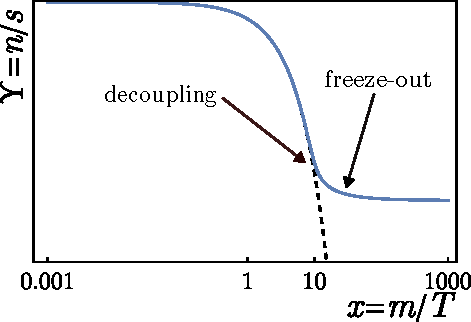
\includegraphics[scale=1]{Images/wimp_decoupling.pdf}
\caption{\hspace{0.1in}Desacoplamiento del plasma primordial y \textit{freeze-out} de un WIMP.}
\label{wimp}
\end{figure}


